%%%%%%%%%%%%%%%%%%%%%%% file template.tex %%%%%%%%%%%%%%%%%%%%%%%%%
%
% This is a general template file for the LaTeX package SVJour3
% for Springer journals.          Springer Heidelberg 2010/09/16
%
% Copy it to a new file with a new name and use it as the basis
% for your article. Delete % signs as needed.
%
% This template includes a few options for different layouts and
% content for various journals. Please consult a previous issue of
% your journal as needed.
%
%%%%%%%%%%%%%%%%%%%%%%%%%%%%%%%%%%%%%%%%%%%%%%%%%%%%%%%%%%%%%%%%%%%
%
% First comes an example EPS file -- just ignore it and
% proceed on the \documentclass line
% your LaTeX will extract the file if required
\begin{filecontents*}{example.eps}
%!PS-Adobe-3.0 EPSF-3.0
%%BoundingBox: 19 19 221 221
%%CreationDate: Mon Sep 29 1997
%%Creator: programmed by hand (JK)
%%EndComments
gsave
newpath
  20 20 moveto
  20 220 lineto
  220 220 lineto
  220 20 lineto
closepath
2 setlinewidth
gsave
  .4 setgray fill
grestore
stroke
grestore
\end{filecontents*}
%
\RequirePackage{fix-cm}
%
%\documentclass{svjour3}                     % onecolumn (standard format)
%\documentclass[smallcondensed]{svjour3}     % onecolumn (ditto)
\documentclass[smallextended]{svjour3}       % onecolumn (second format)
%\documentclass[twocolumn]{svjour3}          % twocolumn
%
\smartqed  % flush right qed marks, e.g. at end of proof
%
\usepackage{graphicx}
%
% \usepackage{mathptmx}      % use Times fonts if available on your TeX system
%
% insert here the call for the packages your document requires
%\usepackage{latexsym}
% etc.
%

%
\smartqed  % flush right qed marks, e.g. at end of proof
%
\usepackage{graphicx}
\usepackage{amssymb}
\usepackage{amsmath}
\usepackage{clrscode}
\usepackage{url}


% please place your own definitions here and don't use \def but
% \newcommand{}{}
%
% Insert the name of "your journal" with
% \journalname{Mathematical Programming A}
%
\begin{document}

\title{Bipartite modularity maximization: complexity and exact methods%\thanks{Grants or other notes
%about the article that should go on the front page should be
%placed here. General acknowledgments should be placed at the end of the article.}
}
%\subtitle{Do you have a subtitle?\\ If so, write it here}

%\titlerunning{Short form of title}        % if too long for running head

\author{Alberto Costa         \and
        Pierre Hansen          \and %etc.
        Fabio Roda \and
        Manuel Ruiz
}

%\authorrunning{Short form of author list} % if too long for running head

\institute{A. Costa \at
              Singapore University of technology and Design, 138682 Singapore   \\
              %Tel.: +123-45-678910\\
              %Fax: +123-45-678910\\
              \email{costa@sutd.edu.sg}           %  \\
%             \emph{Present address:} of F. Author  %  if needed
           \and
           P. Hansen \at
              GERAD, HEC Montr\'eal, 3000 Chemin de la C\^ote-Sainte-Catherine, H3T 2A7 Montr\'eal, Canada \\
              \email{pierre.hansen@gerad.ca}
              \and
              F. Roda \at
              LIX, \'Ecole Polytechnique, F-91128 Palaiseau, France  \\
              %CESAMES, 75002 Paris, France\\
              %Tel.: +123-45-678910\\
              %Fax: +123-45-678910\\
              \email{roda@lix.polytechnique.fr}           %  \\
             \and
             M. Ruiz \at
             Artelys, 75002 Paris, France\\
            \email{manuel.jean.ruiz@gmail.com}
}

\date{Received: date / Accepted: date}
% The correct dates will be entered by the editor


\maketitle

\begin{abstract}
Clustering has been a subject of intense study in the last decades. Its aim is to find subsets of vertices, called clusters, which are more likely to be joined pairwise by an edge than vertices in different clusters. 
A famous method to formalize this idea is the maximization of the modularity, which represents the fraction of edges within the clusters minus the expected fraction of such edges in a random graph with the same distribution of degrees.  
Modularity has been recently extended to bipartite graphs, which can be used to represent many situations (e.g., recommender systems between users and items, information retrieval with documents and terms, graphs showing relationships between authors and papers). This paper shows that maximizing the bipartite modularity is NP-hard. Moreover, some mathematical programming exact formulations are presented, as well as the column generation extension. Results for some instances of the literature are reported.
\keywords{Bipartite graphs \and Clustering \and Modularity maximization}
% \PACS{PACS code1 \and PACS code2 \and more}
% \subclass{MSC code1 \and MSC code2 \and more}
\end{abstract}


\section{Introduction}
Clustering on graphs is a very important topic, which has been studied under different points of view during these last years. Given a graph $G=(V,E)$, where $V$ is the set of vertices and $E$ is the set of edges joining pair of vertices, clustering aims at finding partitions of $G$, where a partition is a split of $V$ into disjoint pairwise nonempty subsets of vertices covering $V$, called clusters, where the vertices belonging to the same cluster are more likely to be connected pairwise than to vertices belonging to other clusters. In order to formalize this idea, different approaches were proposed. 
For example, one could specify some conditions that must be satisfied by each cluster of the partition. In \cite{Radicchi} the authors proposed the concepts of cluster in the \emph{strong} and \emph{weak} sense: the former refers to a cluster $C$ where, for each vertex belonging to $C$, the number of its neighbors within $C$ is larger than the number of its neighbors outside $C$. In the latter the sum, for all the vertices belonging to $C$, of the difference between the number of neighbors within $C$ and the number of neighbors outside $C$ is positive. Recently a modified version of the strong criterion, called \emph{almost-strong}, has been proposed in \cite{PhysRevE.85.046113}: for each degree 2 vertex $v_i$ the strong condition forces this vertex and its 2 neighbors $v_j$ and $v_k$ to be in the same cluster, even if $v_j$ and $v_k$ are connected to two eterogeneous sets of vertices. The almost-strong criterion is the same as the strong one, exept for each degree 2 vertex $v_i$, where it is sufficient that at least one between $v_j$ and $v_k$ is in the same cluster as $v_i$. Other criterion have been proposed in \cite{wasserman1994,PhysRevE.78.026121,1082924}.

Alternatively, one can define an objective function to maximize or minimize. 

In this paper we consider the so called modularity maximization, introduced in.

\section{Problem definition}

\section{Complexity}

\section{Mathematical programming models for bipartite modularity maximization}

\subsection{Fortet based formulation}
\subsection{Binary decomposition formulation}
\subsection{Clique partitioning based formulation} 

\section{Column generation}

\section{Computational results}

\section{Conclusions}

























% For one-column wide figures use
%\begin{figure}
% Use the relevant command to insert your figure file.
% For example, with the graphicx package use
  %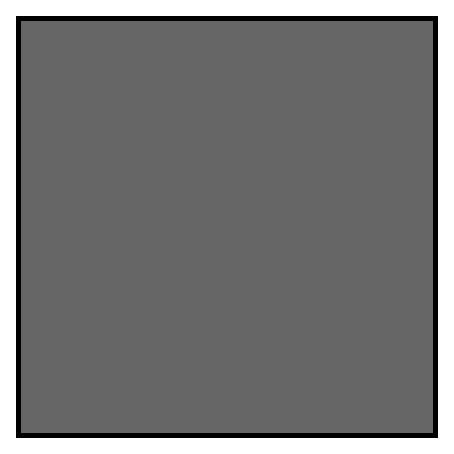
\includegraphics{example.eps}
% figure caption is below the figure
%\caption{Please write your figure caption here}
%\label{fig:1}       % Give a unique label
%\end{figure}
%
% For two-column wide figures use
%\begin{figure*}
% Use the relevant command to insert your figure file.
% For example, with the graphicx package use
  %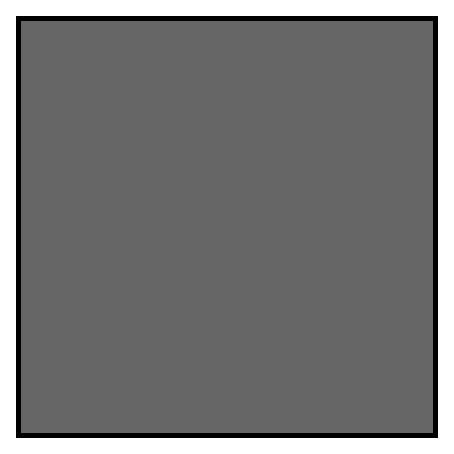
\includegraphics[width=0.75\textwidth]{example.eps}
% figure caption is below the figure
%\caption{Please write your figure caption here}
%\label{fig:2}       % Give a unique label
%\end{figure*}
%
% For tables use
%\begin{table}
% table caption is above the table
%\caption{Please write your table caption here}
%\label{tab:1}       % Give a unique label
% For LaTeX tables use
%\begin{tabular}{lll}
%\hline\noalign{\smallskip}
%first & second & third  \\
%\noalign{\smallskip}\hline\noalign{\smallskip}
%number & number & number \\
%number & number & number \\
%\noalign{\smallskip}\hline
%\end{tabular}
%\end{table}


\begin{acknowledgements}
A. C. has been partially supported by IDC Grant IDSF1200101OH.
\end{acknowledgements}

% BibTeX users please use one of
%\bibliographystyle{spbasic}      % basic style, author-year citations
\bibliographystyle{spmpsci}      % mathematics and physical sciences
%\bibliographystyle{spphys}       % APS-like style for physics
\bibliography{bibliografia}   % name your BibTeX data base

% Non-BibTeX users please use
%\begin{thebibliography}{}
%
% and use \bibitem to create references. Consult the Instructions
% for authors for reference list style.
%
%\bibitem{RefJ}
% Format for Journal Reference
%Author, Article title, Journal, Volume, page numbers (year)
% Format for books
%\bibitem{RefB}
%Author, Book title, page numbers. Publisher, place (year)
% etc
%\end{thebibliography}

\end{document}
% end of file template.tex

